% This work is made available under the terms of the
% Creative Commons Attribution-ShareAlike 4.0 license,
% http://creativecommons.org/licenses/by-sa/4.0/.
%
% Version: $Revision$

\chapter{Clustering}
\label{clustering}
Clustering behaves very much like Classification/Regression, the only difference
being that it is an unsupervised learning process. This means that the flows
won't contain a \textit{WekaClassSelector} actor to set the class attribute in
the loaded data. Due to the similarity, the section here will cover only
the basics of clustering.

\section{Building models}
Building clustering models is as easy as building classification/regression
models. Instead of the \textit{WekaTrainClassifier} transformer, you use the
\textit{WekaTrainClusterer} one. Similar, you use a \textit{WekaClustererSetup}
source instead of the \textit{WekaClassifierSetup} one to define (and output)
a clusterer setup, placed inside a \textit{CallableActors} standalone.

Figures \ref{build_clusterer-flow} and \ref{build_clusterer-output} show a flow
\footnote{adams-weka-build\_clusterer.flow} that builds a \textit{SimpleKMeans}
clusterer on a dataset (the class attribute gets removed using a
\textit{WekaFilter} actor) and the generated model gets displayed.

\begin{figure}[ht]
  \begin{minipage}[t]{0.5\linewidth}
    \centering
    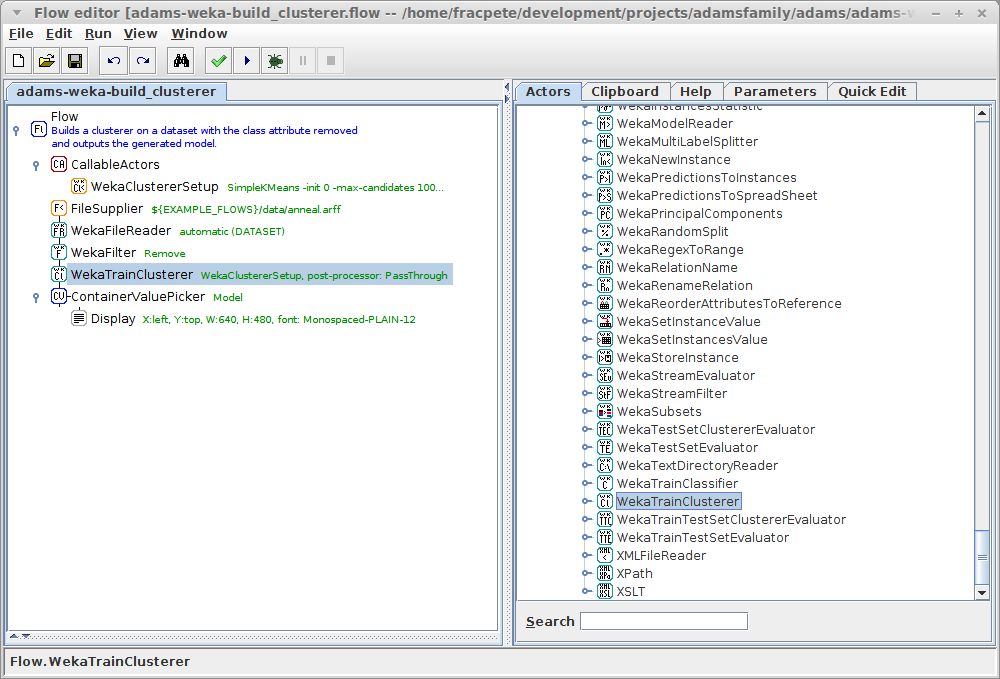
\includegraphics[width=6.0cm]{images/build_clusterer-flow.png}
    \caption{Building a clusterer and outputting the model.}
    \label{build_clusterer-flow}
  \end{minipage}
  \hspace{0.5cm}
  \begin{minipage}[t]{0.5\linewidth}
    \centering
    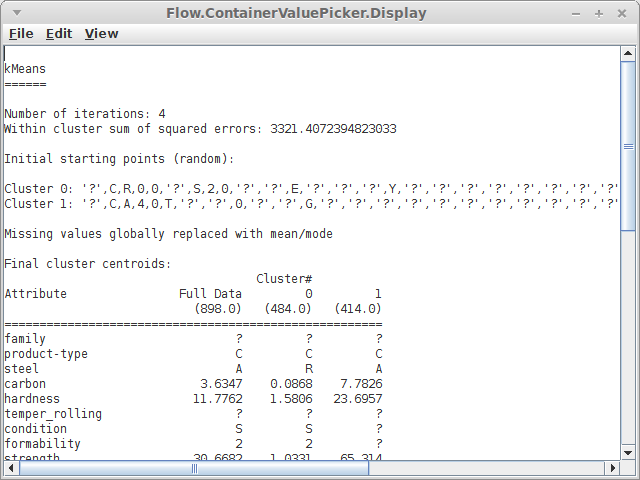
\includegraphics[width=5.5cm]{images/build_clusterer-output.png}
    \caption{Cluster model output.}
    \label{build_clusterer-output}
  \end{minipage}
\end{figure}

If the base cluster algorithm is an incremental one, i.e., one that implements
the \textit{weka.clusterers.UpdateableClusterer} interface, you can build your
clustering model incrementally as well. The flow
\footnote{adams-weka-build\_clusterer\_incrementally.flow} in Figure
\ref{build_clusterer_incrementally-flow} builds the CobWeb cluster algorithm
incrementally and outputs the generated models every 25 instances (see Figure
\ref{build_clusterer_incrementally-output}).

\begin{figure}[ht]
  \begin{minipage}[t]{0.5\linewidth}
    \centering
    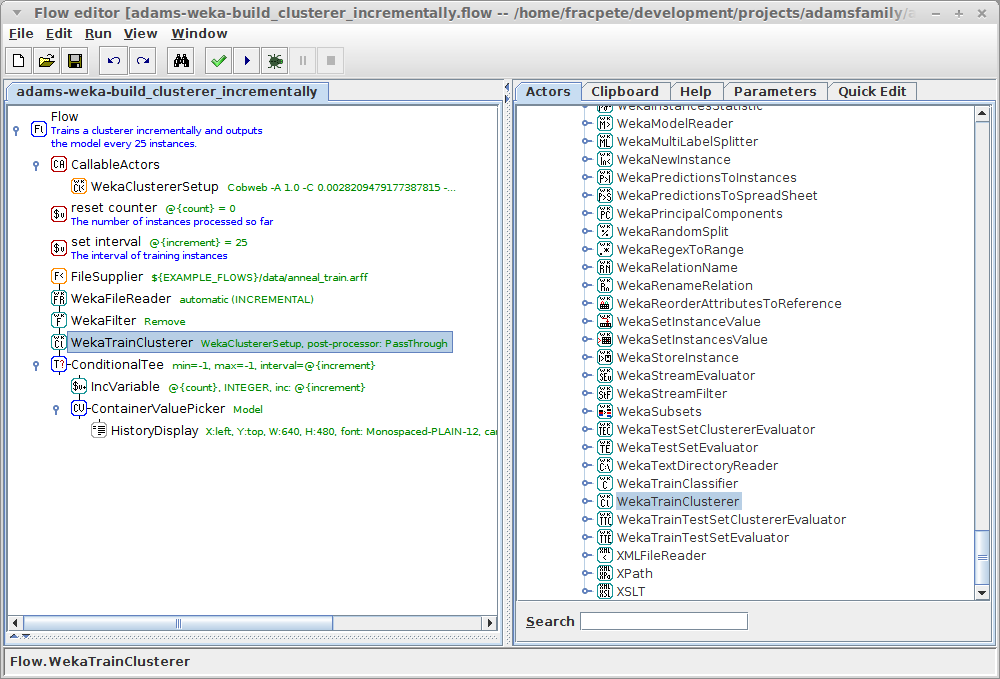
\includegraphics[width=6.0cm]{images/build_clusterer_incrementally-flow.png}
    \caption{Building a clusterer incrementally and outputting the model.}
    \label{build_clusterer_incrementally-flow}
  \end{minipage}
  \hspace{0.5cm}
  \begin{minipage}[t]{0.5\linewidth}
    \centering
    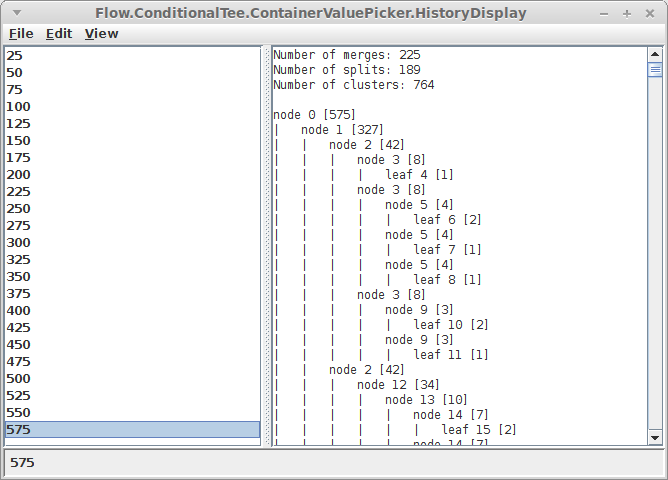
\includegraphics[width=5.5cm]{images/build_clusterer_incrementally-output.png}
    \caption{Cluster model outputs, generated every 25 instances.}
    \label{build_clusterer_incrementally-output}
  \end{minipage}
\end{figure}

\section{Evaluating clusterers}
ADAMS offers transformers for evaluation clusterers on data similar to the 
ones for classification:
\begin{tight_itemize}
	\item \textit{WekaClusterAssignments} - outputs the cluster assignments
	from the last evaluation (if available).
	\item \textit{WekaClusterEvaluationSummary} - generates a string representation
	of a cluster evaluation (or container)
	\item \textit{WekaCrossValidationClustererEvaluator} - cross-validates a
	clusterer on a dataset, generates log-likelhood.
	\item \textit{WekaTestSetClustererEvaluator} - evaluates a built clusterer
	on a test set.
	\item \textit{WekaTrainTestSetClustererEvaluator} - builds and evaluates
	a clusterer on the training and test set from a train/test-set container.
\end{tight_itemize}

\section{Clustering data}
Clustering new data is done using the \textit{WekaClustering} transformer, which
takes a single instance as input and outputs the generated clustering
information in form of a container (\textit{WekaClusteringContainer}). You can
either specify a serialized clusterer model to use or a callable actor to obtain
the clusterer from. The flow \footnote{adams-weka-clustering\_data.flow} in
Figure \ref{clustering-flow} shows how to build a clusterer and use it to
cluster new data, outputting the cluster distributions (see Figure
\ref{clustering-output} for the generated output).

\begin{figure}[ht]
  \begin{minipage}[t]{0.5\linewidth}
    \centering
    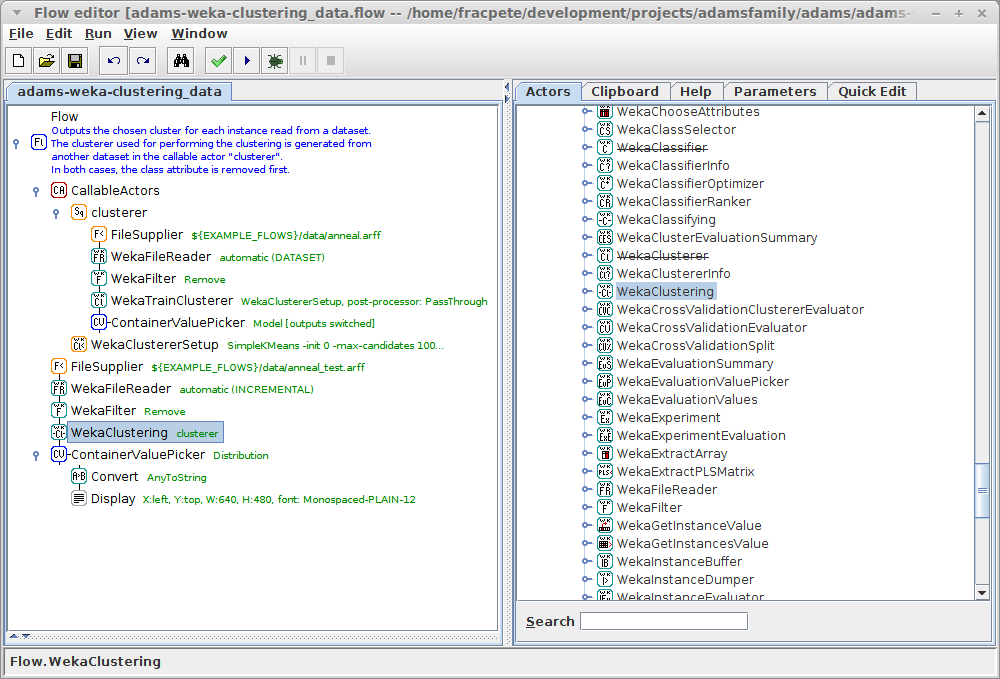
\includegraphics[width=6.0cm]{images/clustering-flow.png}
    \caption{Flow for clustering new data.}
    \label{clustering-flow}
  \end{minipage}
  \hspace{0.5cm}
  \begin{minipage}[t]{0.5\linewidth}
    \centering
    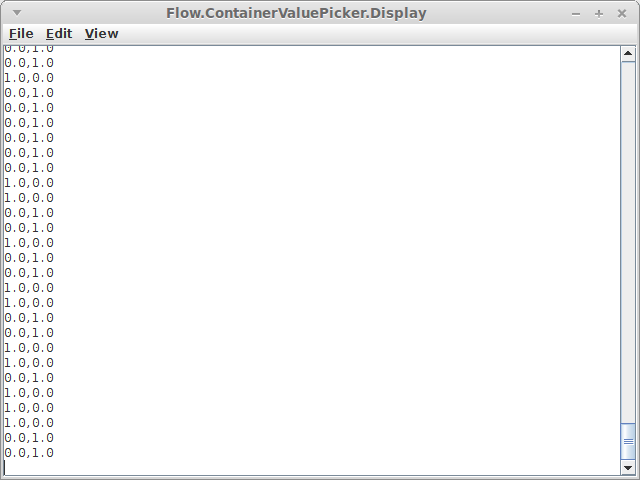
\includegraphics[width=5.5cm]{images/clustering-output.png}
    \caption{Generated cluster.}
    \label{clustering-output}
  \end{minipage}
\end{figure}
